\subsection{Page allocator}

\begin{frame}[fragile]
  \frametitle{Pages and page blocks}

  \begin{itemize}
  \item Linux manages memory in units of pages.
    \begin{itemize}
    \item Typically \unit[4]{KiB} in size.
    \end{itemize}
  \item Page can have order ranging from 0 to 10.\footnote{Strictly
    speaking, from zero to one less than \lstinline|MAX_ORDER| which is
    usually 11.}
    \begin{itemize}
    \item $n$-order page consists of $2^n$ \unit[4]{KiB} pages.
    \item 10-order page is called max-order page.
    \end{itemize}
  \item Pages are grouped into page blocks.
  \item Page block consists of 1024 pages, same size as max-order
    page.\footnote{This actually depends, but it's the case for ARM
      and x86.}
  \item {\footnotesize Let's forget about zones or NUMA.}
  \end{itemize}
\end{frame}

\begin{frame}
  \frametitle{Pages and page blocks, cont}
  \begin{centering}
  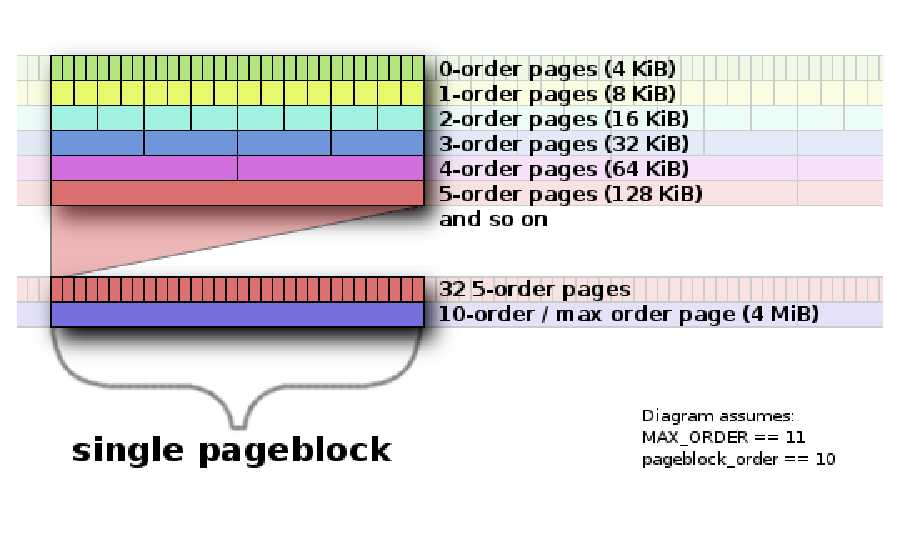
\includegraphics[width=0.9\textwidth]{build/pages.eps}
  \end{centering}
\end{frame}


\begin{frame}[fragile]
  \frametitle{Migrate types}

  \begin{itemize}
  \item On allocation, user requests an unmovable, a~reclaimable or
    a~movable page.
    \begin{itemize}
    \item For our purposes, we treat reclaimable as unmovable.
    \end{itemize}
  \item Movable pages will be set up so that they can be migrated.
  \end{itemize}

  \begin{itemize}
  \item To try keep pages of the same type together, each free page
    and each page block has a~migrate type assigned.
  \item But allocator will use fallback types.
  \item And migrate type of a~free page and page blocks can change.
  \end{itemize}
\end{frame}

\begin{frame}
  \frametitle{Buddy allocator}

  \begin{itemize}
  \item Page allocator uses buddy allocation algorithm.
    \begin{itemize}
    \item Hence different names: buddy system or buddy allocator.
    \end{itemize}
  \item
  \end{itemize}
\end{frame}
